Alternatively, the constrained optimization problem \eqref{eq:disoTPS_YB_move_standard} can be solved via two successive SVDs with an optional disentangling prodcedure with the goal of reducing the truncation error or some entanglement measure. This is the same algorithm that was used for the MM in the original isoTPS \cite{cite:efficient_simulation_of_dynamics_in_two_dimensional_quantum_spin_systems}. The algorithm is sketched in figure \figref{fig:yb_move_svd_disent} and is made up of three main steps.
\begin{enumerate}
	\item We start by contracting the tensors $T$, $W_1$ and $W_2$ into a single tensor $\Psi$. This tensor is then split from left to right via a truncated SVD
	\begin{equation}
		\Psi = XSZ^\dagger = X\left(SZ^\dagger\right) \eqqcolon X\theta
	\end{equation}
	as shown in figure \figref{fig:yb_move_svd_disent}(a). The bond dimension is truncated to $D^2$.
	\item Next, we split the index of the bond connecting $X$ and $\theta$ into two indices of dimension $D$ each, see figure \figref{fig:yb_move_svd_disent}(b). To proceed, we note that there exists a degree of freedom on the bonds connecting $X$ and $\theta$: A unitary $U$ and its adjoint can be inserted as shown in the second step of figure \figref{fig:yb_move_svd_disent}(b) without changing the result of the contraction
	\begin{equation}
		XU^\dagger U\theta = \left(XU^\dagger\right)\left(U\theta\right) \eqqcolon T^\prime \tilde{\theta}.
	\end{equation}
	This unitary $U$ can be chosen to minimize the truncation error of the next step by \textit{disentangling} the tensor $\theta$. We will discuss procedures of finding such a \textit{disentangling unitary} on the next page.
	\item In the last step, the tensor $\tilde{\theta}$ is split vertically into $W_1^\prime$ and $W_2^\prime$ using a truncated SVD as shown in figure \figref{fig:yb_move_svd_disent}(c). Here, the bond dimension is truncated to $\chi$. We end up with the three tensors $T^\prime$, $W_1^\prime$ and $W_2^\prime$, completing the YB move.
\end{enumerate}
Before we discuss the disentangling procedure, two comments about step two of the above algorithm are in order. Firstly, there exists a degree of freedom for splitting the bond index, because applying the same permutations to the columns of $X$ and rows of $\theta$ does not change the result of contracting the network. However, this degree of freedom is fixed by the disentangling process, making the exact permutation of the bond splitting irrelevant. Secondly, note that near the edges of the lattice it can happen that the matrizized tensor $\Psi$ has $\tilde{\chi} < D^2$ rows. In this case, the bond dimension after the SVD will also be $\tilde{\chi}$ and we cannot simply split the bond into two bonds of dimension $\chi_1=\chi_2=D$. Instead, we choose a splitting $\chi_1 \le D$, $\chi_2 \le D$ such that $\chi_1\cdot\chi_2$ is maximized, while it must still hold $\chi_1\cdot\chi_2\le\tilde{\chi}$. We additionally prefer "equal" splittings $\chi_1\approx\chi_2\approx\sqrt{\tilde{\chi}}$ if possible. One can find such a splitting easily by computing all possible combinations of $\chi_1$ and $\chi_2$ and keeping only the best one. This has a computational cost of $\mathcal{O}\left(\sqrt{\tilde{\chi}}\right) = \mathcal{O}\left(D\right)$. \par
\begin{figure}
	\centering
	\includegraphics[width=0.8\textwidth]{figures/Tensor_Networks/yb_move_svd_disent.jpeg}
	\caption{test\todo{Write caption.}}
	\label{fig:yb_move_svd_disent}
\end{figure}
\subsubsection*{The disentangling process}
We will now discuss the problem of finding a good disentangling unitary $U$ for step 2 of the above algorithm, which is crucial for the performance of the YB move. The problem can be formulated as follows: Given the tensor $\theta$ that is obtained after splitting the index in step two, find a unitary $U$ minimizing a cost function $f(U, \theta)$. In the following, let $S_j$, $j = 1, \dots, \chi D^2$ be the singular values of the SVD $\tilde{\theta} = U\theta = USV^\dagger$, see figure \ref{}. We discuss two cost functions, namely the truncation error
\begin{equation}
	f_\text{trunc}\left(U, \theta\right) = 
\end{equation}

\begin{figure}
	\centering
	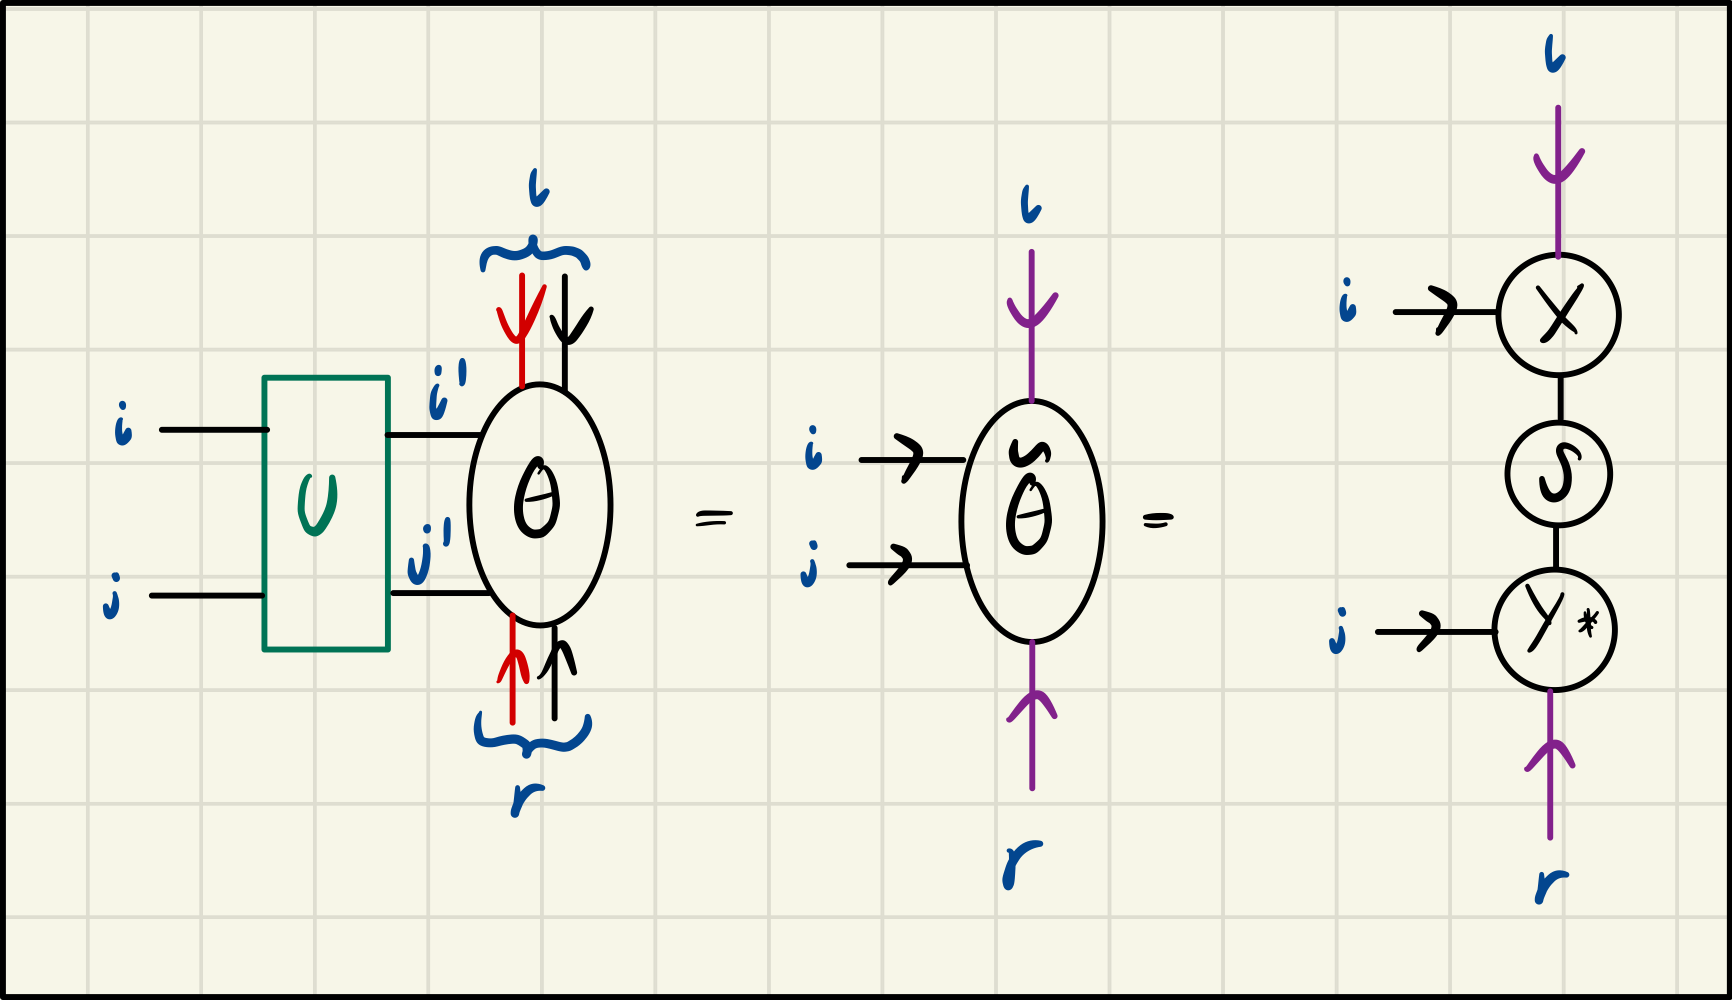
\includegraphics[width=0.8\textwidth]{figures/disoTPS/disentangling_theta_definition.jpeg}
	\caption{The disentangling unitary $U$ is contracted with the wave function tensor $\theta$ to form $\tilde{\theta}$, which is subsequently split via an SVD $\tilde{\theta} = XSY^\dagger$.}
	\label{fig:disentangling_theta_definition}
\end{figure}

\begin{figure}
	\centering
	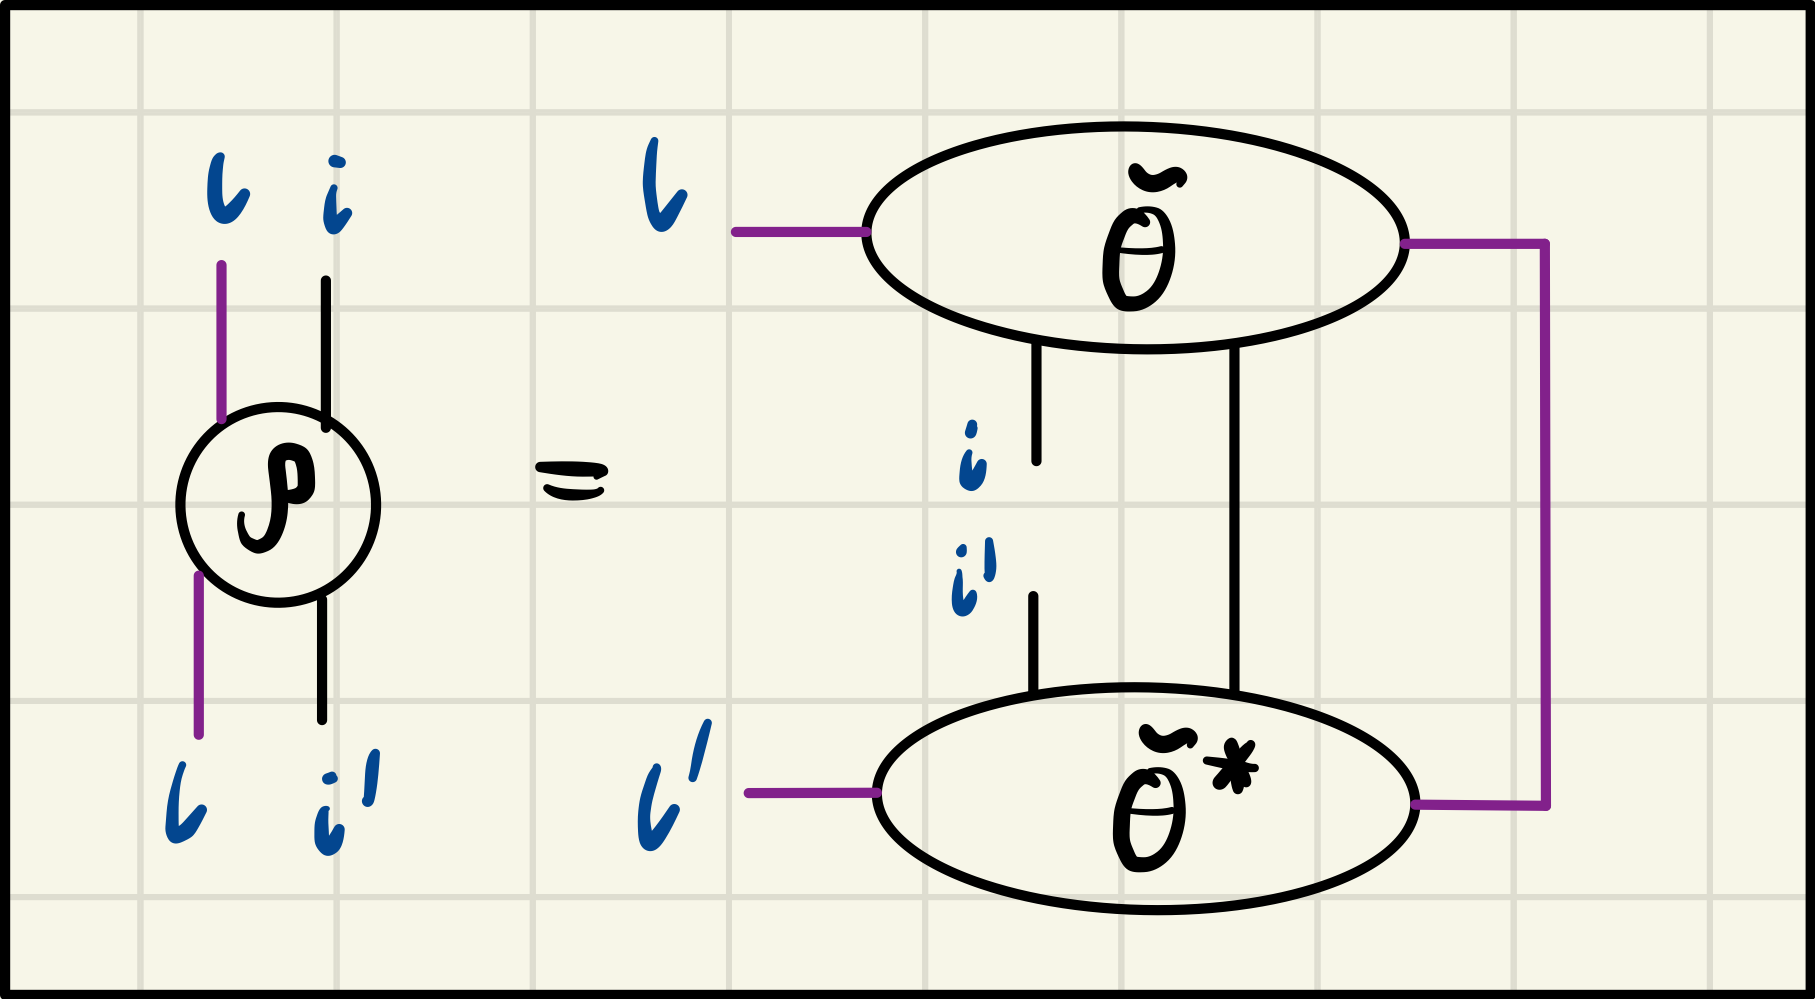
\includegraphics[width=0.8\textwidth]{figures/disoTPS/disentangling_rho_definition.jpeg}
	\caption{Definition of the reduced density matrix $\rho$.}
	\label{fig:disentangling_rho_definition}
\end{figure}

\begin{figure}
	\centering
	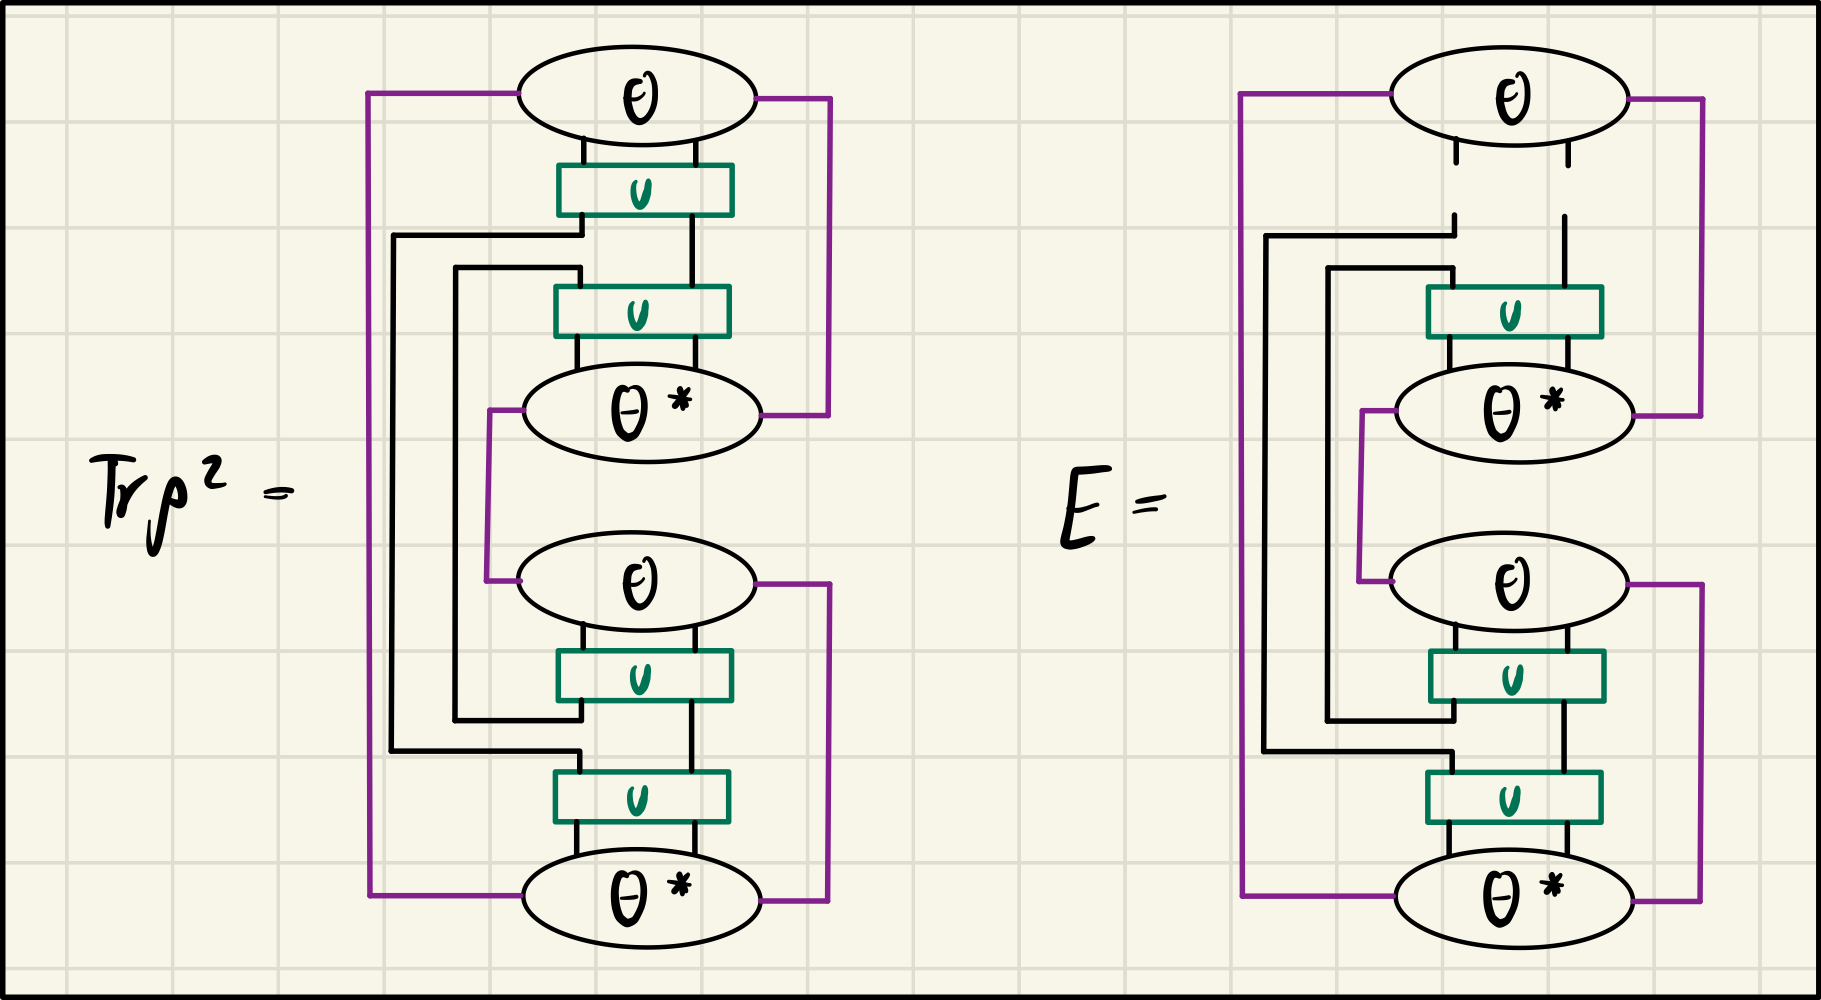
\includegraphics[width=0.8\textwidth]{figures/disoTPS/disentangling_evenbly_vidal_algorithm.jpeg}
	\caption{(a) Tensor network for the computation of the cost function \eqref{}. (b) Taking out one unitary $U$, the tensor network is contracted into the environment $E$.}
	\label{fig:disentangling_evenbly_vidal_algorithm}
\end{figure}

\begin{figure}
	\centering
	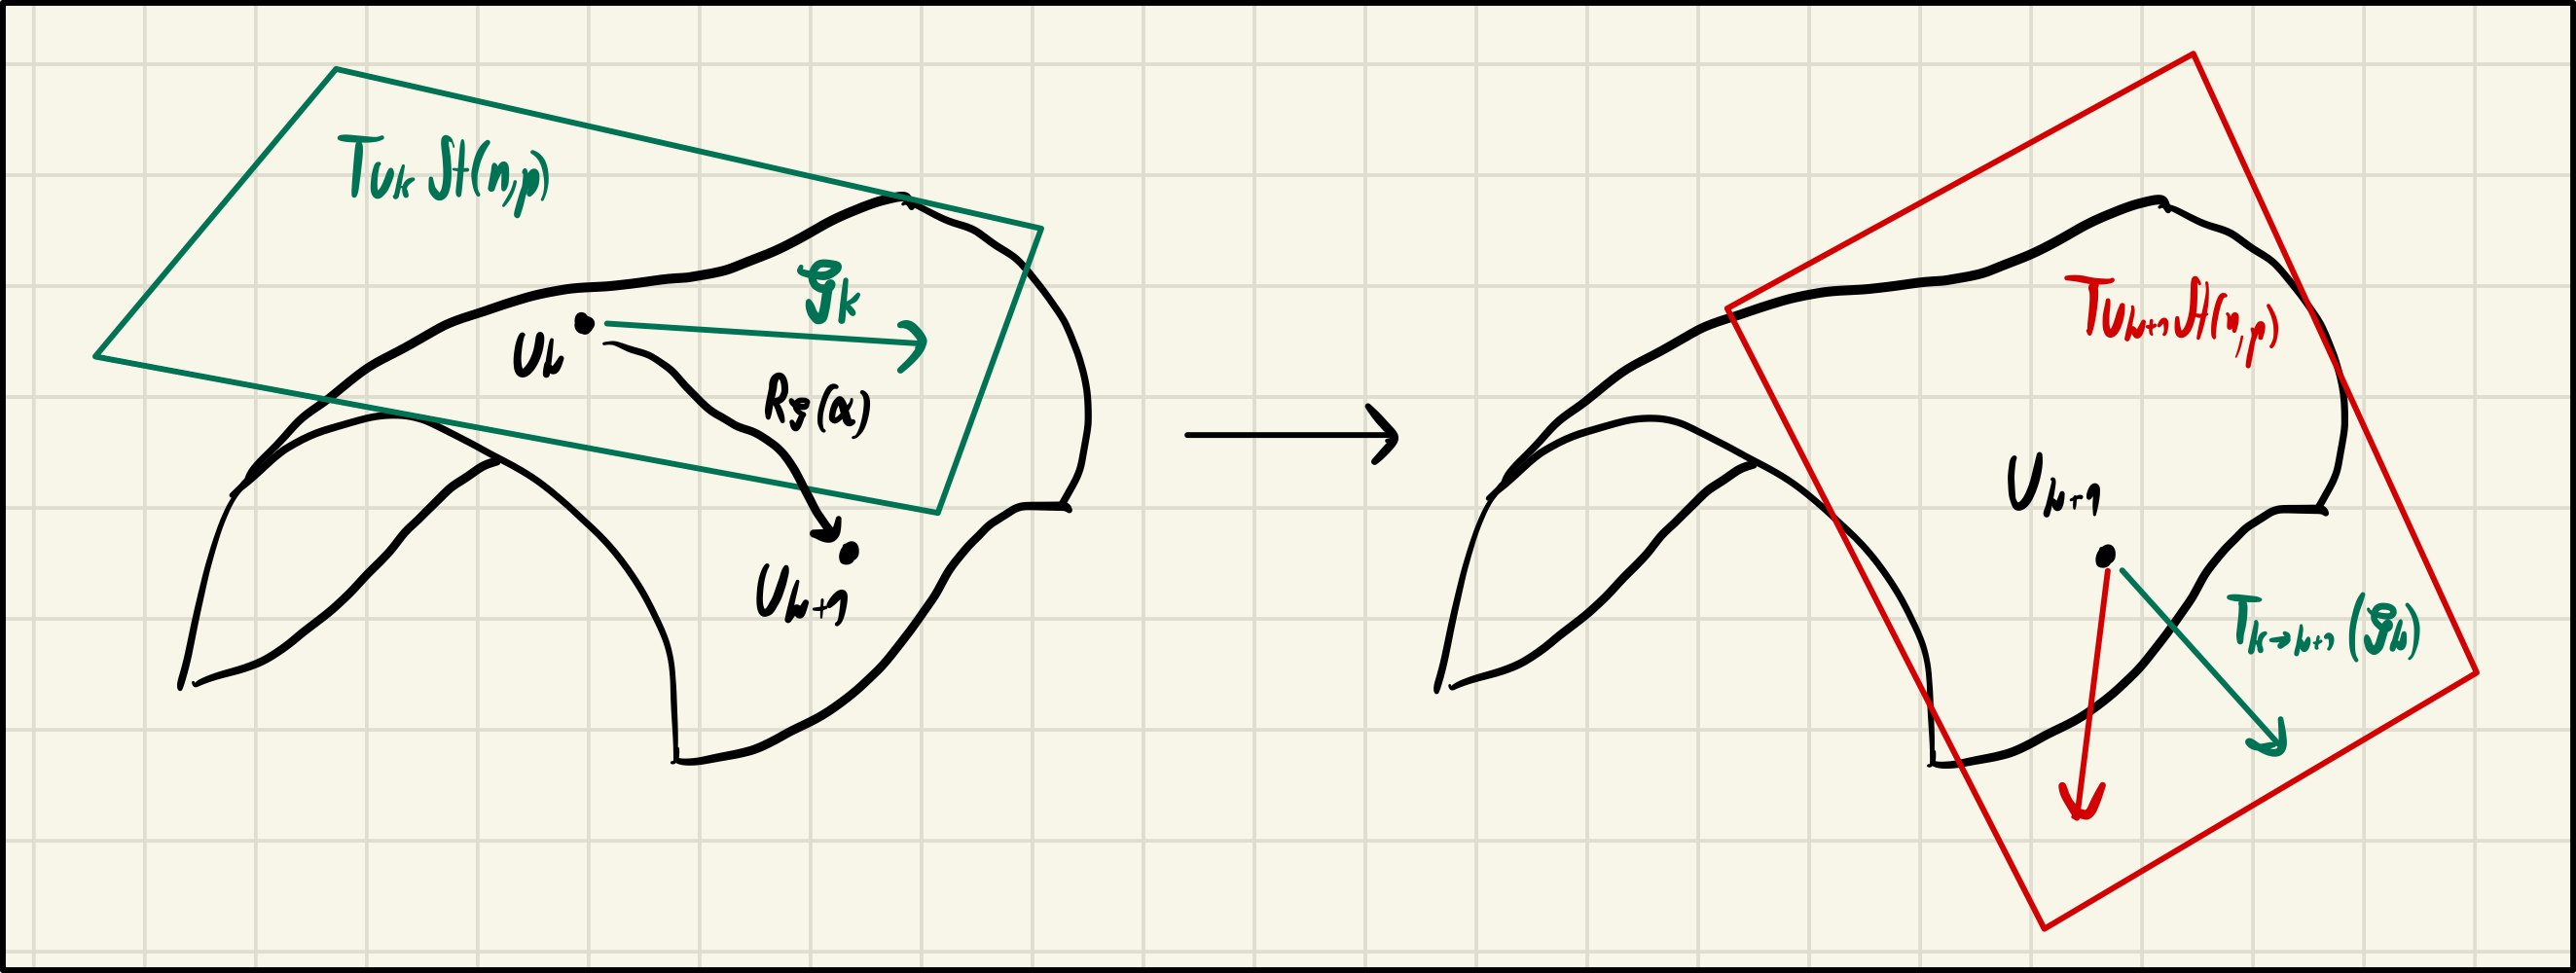
\includegraphics[width=0.8\textwidth]{figures/disoTPS/disentangling_riemannian_optimization.jpeg}
	\caption{In this figure, a visualization of optimization on Riemannian manifolds is given. The iterate $U_k$ (left) is updated along the search direction $\xi_k$, which is an element of the tangent space $T_{U_k}\Stiefel$. The next iterate $U_{k+1}$ is computed with the retraction $R_\xi\left(\alpha\right)$, where $\alpha\in\mathbb{R}$ is the step size. For the computation of the next search direction $\xi_{k+1}$ the previous search direction $\xi_k$ is needed, which is brought to the tangent space $T_{U_{k+1}}\Stiefel$ of the new iterate $U_{k+1}$ via the vector transport $T_{k\rightarrow k+1}\left(\xi_k\right)$.}
	\label{fig:disentangling_riemannian_optimization}
\end{figure}